%
% einleitung.tex -- Beispiel-File für die Einleitung
%
% (c) 2020 Prof Dr Andreas Müller, Hochschule Rapperswil
%
% !TEX root = ../../buch.tex
% !TEX encoding = UTF-8
%
\section{Fakultät erweitern\label{gamma:section:teil0}}
\kopfrechts{Fakultät erweitern}

Die Fakultät ist definiert als
\begin{equation}
n! = \prod_{k=1}^{n} k = 1 \cdot 2 \cdot 3 \cdot \ldots \cdot n
\label{gamma:fakultaet}
\end{equation}
und gilt für die natürlichen Zahlen. Sie fällt vorallem durch ihr schnelles Wachstum auf.
Nicht ganz intuitiv dabei ist, dass $0! = 1$ ist. Stellt man die Fakultät in die rekursive Form um
\begin{equation}
n! = n \cdot (n-1)! \leftrightarrow (n-1) = n!/n
\label{gamma:fakultaet-rekursiv}
\end{equation}
und setzte 0 für $(n-1)$ ein, zeigt sich warum $0! = 1!/1 = 1$ ist. 

Eine erste Definition der Fakultät für nicht natürliche Zahlen wird bereits 1720 von Daniel Bernoulli und Christian Goldbach gegeben. 
Auch Leonhard Euler und James Stirling steuern im Laufe der Jahrhunderte ihre eigene Definition bei. 
Man sieht, die Erweiterung der Fakultät hat grosse Namen der Mathematik beschäftigt. 

\subsection{Bohr-Mullerup Theorem}

Umeine Funktion zu finden, welche die Fakultät erweitert, wird das Bohr-Mullerup Theorem verwendet. 
Erfüllt eine Funktion alle drei Eigenschaften, kann sie als Erweiterung der Fakultät für nicht natürliche Zahlen betrachtet werden.
\begin{enumerate}
  \item $f(1) = 1$
  \item $f(x+1) = x \cdot f(x), x > 0$
  \item $f(x)$ ist logarithmisch konvex.
\end{enumerate}

Die erste Eigenschaft ist dabei selbsterklärend.
Die zweiten Eigenschaft verlangt, dass die Funktion rekursiv definiert werden kann. 
Beispielsweise die Fakultät erfüllt das, da $5! = 5 \cdot 4!$ ist.
Die dritte Eigenschaft verlangt logarithmisch Konvexität, was auch als "wächst schnell" verstanden werden kann.

\subsubsection{Logarithmische Konvexität}

Eine Kurve ist konvex, wenn diese nach oben geöffnet ist, beispielsweise $f(x) = x^2$. 
Von logarithmischer Konvexität spricht man, wenn nach der Anwendung des Logarithmus, die resultierende Funktion auch Konvex ist.
Bildlich gezeigt am Beispiel $g(x) = e^{x^2} $. 
Nach Anwendung des natürlichen Logarithmus, ergibt sich die $\ln(g(x)) = x^2$.
Die Funktion $x^2$ ist weiterhin nach oben geöffnet, womit $g(x)$ logarithmisch komplex ist.

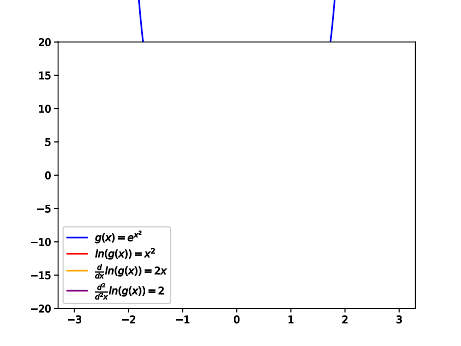
\includegraphics[width=0.4\textwidth]{papers/gamma/img/log_convex_3.png} %fix picture and size, lol

\subsubsection{Suche nach einer passenden Funktion}

Eine Funktion welche Eigenschaften eins und zwei erfüllt, lässt sich verhältnismässig leicht finden.
Nimmt man die Funktion $f(x) = 2\sin(2\pix)+1$, wird Eigenschaft 1 durch den Shift nach rechts und die Rekursitivät durch die Periode des Sinus erfüllt.
Wie die Grafik TODO ADD LINK zeigt, lässt sich damit die Funktion zeichen die durch die bekannten Fakultät-Werte geht.
Die Ausschläge der Funktion nach unten und oben zeigen grafisch, dass die logarithmische Konvexität für diese Funktion nicht gegeben sein kann.

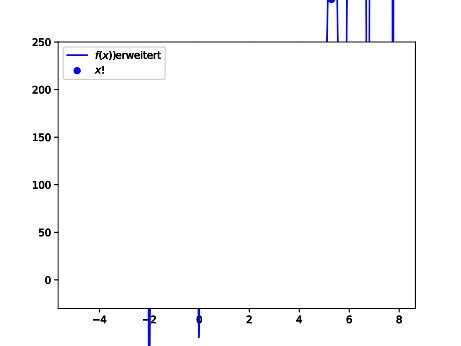
\includegraphics[width=0.4\textwidth]{papers/gamma/img/sin_extended.png}

Gesucht wird eine Funktion, welche alle drei Eigenschaften der Fakultät erfüllt. Wie die Quelle (TODO: ADD QUELLE) beweist, werden alle Eigenschaften lediglich von der Gamma-Funktion erfülllt.